\documentclass[12pt,a4paper]{amsart}

\usepackage{amsmath}
\usepackage{graphicx}
\usepackage{amsrefs}
\usepackage{parskip}
\setlength{\parskip}{0.8em}

\title{Classical and Quantum Chaos: Project Plan}
\author{Benjamin Mason}

\begin{document}

\maketitle

% \section{Questions}

% THE QUESTIONS I WANT ANSWERS TO:

% 1. why is the study of chaos important in classical systems?

% 2. Why do we quantise the systems to study chaos in quantum mechanics?

% 3. How does chaos happen in iterated maps? (Already got the answer from Schek)

% 4. What classical mechanics is important (talk about Hamiltonian mechanics and then integrable systems, difference between conservative systems and dissapitive systems)

% 5. What are features of chaotic behaviour? (bifucations, perioud doubling)

% 6. What quantifies chaotic behaviour (Lynapov exponent)

\section{Project Context}

\subsection{Chaotic systems}
My project will be in the field of \textit{chaos theory}, particularly in classical and quantum systems. Chaotic systems are a type of non-linear dynamical system that have exhibit behaviours that "appears" random or noisy. However, throughout the centuries, universal features of chaotic systems have been discovered, and now chaos theory explains solutions of equations in a variety of fields such as population dynamics, chemical kinetics and celestial mechanics \cite{chaosARUN}.
% Add comma after "however", could also break up the sentence into two in order to increase readability

As we are concerned with dynamical systems, initial conditions of a state of the system and the evolution of a solution to the equations that govern the system, or a trajectory, become fundamental concepts to utilise. A trajectory can evolve with any rule the dynamical system dictates, the simplest one being evolution with time.

% ONE PARAGRAPH ON QUAL AND QUANT PARTS OF CHAOS (BIFURCATIONS, SENSITIVITY, LYNAPOV EXPONENTS, PERIOUD DOUBLING)

Chaotic behaviour includes concepts such as bifurcation (the splitting of trajectories), aperiodic solutions and the presence of attractors. While not all of these are necessary for a system to be called chaotic, there are more quantitative features that determine a system's behaviour. An important one is the Lyapunov exponent, which can be calculated for a chaotic system and will be (on average) positive. This exponent implies that nearby trajectories will diverge exponentially, which gives rise to the famous "butterfly effect" - the sensitivity to choice of initial conditions. I plan on studying this exponent in more detail, and fully explain this phenomenon.

\subsection{A chaotic example}

Examples of dynamical systems are iterative maps, which have the form $x_{i+1} = f(x_{i})$. These are important as they give us useful insights as to how trajectories of complex systems evolve by studying each iteration of the map \cite{HILBORN}.

Consider the closed mapping: $$x_{i+1} = {\mu} x_{i} (1 - x_{i}) \equiv f(\mu, x_{i}) \label{mapping}$$ on the unit interval $x_{i} \in [0, 1] \  {\forall}i \in \mathbb{N}$. This is called \textit{the logistic equation}, which can be used for biological models such as population growth. The value $\mu$ is a control parameter. There exists fixed points of the map i.e. a point $x^{*}$ such that $x^{*} = f(\mu, x^{*})$. For this mapping, the fixed points are: $$x^{*} = 0 \quad x^{*} = 1 - \frac{1}{\mu}$$ A fixed point has an associated stability, which can be found by analysing the absolute value of the derivative of the function $f(\mu, x)$ evaluated at a given fixed point. A stable or attracting fixed point is such that $|f'(x^{*})| < 1$ and iterations $x_{1} \rightarrow x_{2} \rightarrow \cdots \rightarrow x^{*}$ converge to the fixed point (like the trajectories are "attracted" to the point) \cite{SCHECK}. Considering the non-trivial fixed point of the logistic equation, $|f'(\mu, x^{*})| = |2 - \mu|$ which gives restrictions on the value of $\mu$. Notably, $\mu \leq 4$ so that the mapping remains closed under the interval and the fixed point $x^{*}$ is stable for $1 < \mu < 3$. 

% This behaviour is studied by considering the composition $f \circ f$ of the original mapping. Now $x_{1}^{*}$ and $x_{2}^{*}$ are fixed points of the composition of the map.

However, when $\mu > 3$, the trajectories now oscillate between two attracting points, which can be labelled $x_{1}^{*}$ and $x_{2}^{*}$, and the mapping undergoes a bifurcation, the trajectories are now attracted by two points. As $\mu$ increases, this splitting of trajectories occurs more and more often, leading to the bifurcation diagram shown in Figure \ref{fig:bif}. Analysis of the map can find what values of $\mu$ cause bifurcations. One could say that the behaviour looks "chaotic", that the splitting is random. However, it is a consequence of the system and in this case is predictable.

\begin{figure}[h] 
    \centering
    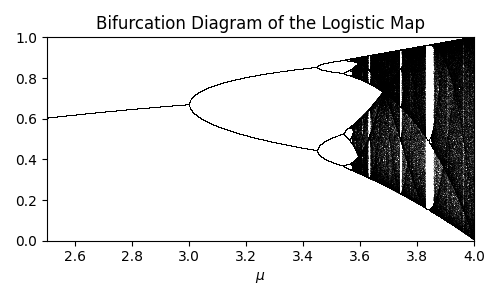
\includegraphics[scale=0.8]{logistic_map_bifur.png}
    \caption{A bifurcation diagram for the logistic map, created in Python by iterating a single trajectory while varying the control parameter $\mu$. The first bifurcation occurs at $\mu$ = 3 as expected.}
    \label{fig:bif}
\end{figure}

\newpage

\subsection{Hamiltonian Mechanics}

The foundations of classical chaos lie in Hamiltonian mechanics. Importantly, the study of \textit{Hamiltonian} or \textit{conservative} systems rather than dissipative systems like ones described by the logistic map. Hamiltonian systems evolve by Hamilton's equations, famously:
$$\dot{q}_{i} = \frac{\partial \mathcal{H}}{\partial p_{i}} \quad \dot{p}_{i} = -\frac{\partial \mathcal{H}}{\partial q_{i}} \quad i = 1, \cdots , N$$
for generalised coordinates $q_{i}(t)$, generalised momenta $p_{i}(t)$ and $N$ degrees of freedom. The \textit{phase space} of the system describes the set of solutions (or states) of the system on a $p$ and $q$ axis. The use of phase space is necessary when describing the evolution of a specific trajectory. If a physical quantity remains constant along a trajectory, then it is called a \textit{constant of the motion}. 

% These are usually named the \textit{action} and \textit{angle} variables, and they are chosen such that they follow a canonical transform of $q$ and $p$ i.e:
% $$\dot{\Theta}_{i} = \frac{\partial \mathcal{H}}{\partial J_{i}} \quad \dot{J}_{i} = -\frac{\partial \mathcal{H}}{\partial \Theta_{i}}$$ and each $J_{i}$ can have an associated function $\Theta_{i}(q, p)$. a canonical transform produces a Hamiltonian

%[REFERENCE HULBORN PG 323]
These constants can always be defined by an action function $J_{i}(q, p)$ \cite{HILBORN}. In the case where such that $\dot{J_{i}} = 0 \ \forall i$, then that system is called \textit{integrable}. An important consequence of this is that there are as many constants of motion as there are degrees of freedom in integrable systems. Thus naturally, a \textit{non-integrable} system has fewer constants of the motions than degrees of freedom. It is these kinds of systems that exhibit chaotic behaviour, and further study is needed into why this is.

 
 % PG 334 LEADS ON TO QUANTUM, RIGHT ST END
 % PG 328 ABOUT WHERE NON-INTEGRABLE SYSTEMS COME UP

\subsection{Billiards}

My project will have a focus on a type of Hamiltonian dynamical system called a \textit{billiard system}. This is a model where a particle moves in a bounded system (such as on the surface of a square) and has perfectly elastic collisions with the boundaries such that energy is a constant of the motion. These systems can be integrable or non-integrable and thus can exhibit normal or chaotic behaviour. 

The classical system has a quantum counterpart. These quantum systems can exhibit quantum chaotic behaviour. I plan on further studying these behaviours to see how they relate to their classical chaotic behaviour. The quantum system has an associated wavefunction, and the exact structure of these wavefunctions will be a focus of my study, specifically if the functions node structure (where the wavefunction equals 0) have the same properties over different billiard systems.

% It is known for many quantum systems, the energy eigenvalues and thus their eigenstates have a definitive order (i.e. ground, 1st excited, etc). This is not necessarily known for billiard systems.
% An example of a Hamiltonian for a billiard system is $$\mathcal{H}(q, p) = \frac{p^{2}}{2m} + V(q)$$ for a potential $V(q)$. This reduces to the free particle Hamiltonian when $V(q)=0$. For a bounded system such as the square, the potential is $V(q) = \inf$ outside the bounded region to gurantee elastic collisions. 



\section{Milestones and Deliverables}

% The general aim of the project is to provide detail into billiard systems, their chaotic nature and study if there are consistent wavefunction node structures for different types of quantum billiard systems. I have split the work into three milestones, with deliverables in each.

\subsection*{Milestone 1: 31/12/24 (End of 2024)}
\begin{itemize}
    \item Understood the basic geometry of chaos in classical systems through studying Hilborn's book \cite{HILBORN} and Scheck's book \cite{SCHECK}.
    \item Understood the set-up of classical billiard systems, and how chaotic behaviour exhibits itself in them through \cite{KORSCH}.
    \item Understood integrable quantum billiard systems, and derived analytical results of their node structure following methods from \cite{ARND} and \cite{CASATI} and other similar work.
\end{itemize}
\subsection*{Milestone 2: 10/03/24 (Start of Week 5)}
\begin{itemize}
    \item Written up the knowledge of the previous semester's research.
    \item Used this research to understand non-integrable quantum billiard systems, and then derived basic numerical results for these systems using package \cite{CODE}.
    \item Analysed the numerical results for evidence of consistent node structure across different systems, to then have submitted the draft project using these first results.
\end{itemize}
\subsection*{Milestone 3: 09/05/25 (End of Week 11)}
\begin{itemize}
    \item Continue to 
\end{itemize}


% I am looking for evidence to see if there is a consistent node structure of excited states of different quantum billiard systems. These systems have classical counterparts so i need to understand fully classical chaos things, like the geometry of chaos, the Poincare sections and mappings, the quantitative features such as Lyanpov exponents and how we calculate them. 

% Then look at how this is quantised, and how quantum chaos behaves. Then look at how to analytically calculate the two dimensional wavefunction for different quantum billiard systems, using research and get a sense of if these integrable systems have consistent node structure, either through boundaries or a node line on the surface. (circular, elliptical, square)

% Then move on to non-integrable quantum billiard systems, and do some numeric to calculate wave functions, and once again see their node structure. 

% CHAOS IN CLASSICAL AND QUANTUM MECHANICS
% SCHECK
% HILBORN
% QUANTUM CHAOS FOR THE VIBRATING RECTANGULAR BILLIARD
% QUANTUM CHAOS FRANK STEINER
% BIB C++ 
\section*{References} 
\begin{biblist}
    \bib{chaosARUN}{book}
    {
      author={Arun V. Holden},
      title={Chaos},
      publisher={Princeton University Press},
      date={2014},
      pages={1},
      isbn={9780691610535},
    }
    
    \bib{HILBORN}{book}
        {
        author = {Robert C. Hilborn},
        year = {1994},
        publisher={Oxford University Press},
        title = {Chaos and Nonlinear Dynamics},
        pages={180}
        }
    \bib{SCHECK}{book}
        {
        author={F Scheck},
        title={Mechanics: From Newton's Laws to Deterministic Chaos},
        publisher={Springer},
        year={1994}, 
        }

    \bib{KORSCH}{book}
        {
        author={Korsch, Hans J{\"u}rgen
        and Zimmer, Frank},
        title={Chaotic Billiards},
        year={2002},
        publisher={Springer Berlin Heidelberg},
        address={Berlin, Heidelberg},
        pages={15--36},
        isbn={978-3-662-04804-7},
        }
    \bib{ARND}{article}
        {
        author = {Backer, Arnd},
        year = {2007},
        month = {06},
        pages = {60 - 64},
        title = {Quantum Chaos in Billiards},
        volume = {9},
        journal = {Computing in Science \& Engineering},
        }

    \bib{CASATI}{article}
    {
        title={The quantum mechanics of chaotic billiards},
       volume={131},
       ISSN={0167-2789},
       number={1–4},
       journal={Physica D: Nonlinear Phenomena},
       publisher={Elsevier BV},
       author={Casati, Giulio and Prosen, Tomaž},
       year={1999},
       month=jul, pages={293–310} 
   }
    \bib{CODE}{article}
    {
        title = {Bill2d — A software package for classical two-dimensional Hamiltonian systems},
        journal = {Computer Physics Communications},
        volume = {199},
        pages = {133-138},
        year = {2016},
        issn = {0010-4655},
        author = {J. Solanpää and P.J.J. Luukko and E. Räsänen},
    }


   

\end{biblist}


\end{document}
